%\VignetteIndexEntry{Answer 05 from Seminar III: R/Bioconductor}
%\VignetteDepends{}
%\VignetteKeywords{R, Bioconductor}
%\VignettePackage{SIII: R/Bioc}
\documentclass[letterpaper,12pt]{article}

%%%%%%%%%%%%%%%%%%%%%%%% Standard Packages %%%%%%%%%%%%%%%%%%%%%%%%%%%%%%%%%%%%%%%%%%
%\usepackage{epsfig}
%\usepackage{graphicx}
%\usepackage{graphics}
%\usepackage{amssymb}
%\usepackage{amsmath}
%\usepackage{mathrsfs}
%\usepackage{caption}
%\usepackage{comment}
\usepackage{fancyvrb}
\usepackage{fancyhdr}

\usepackage[a4paper]{geometry}
\usepackage{hyperref,graphicx}

%\usepackage[spanish]{babel}
%\selectlanguage{spanish}
%\usepackage[utf8]{inputenc}

%%%%%%%%%%%%%%%%%%%%%% some personal commands %%%%%%%%%%%%%%%%%%%%%%%%%%%%%%%%%%%%%%%%%%%%
\newcommand{\pl}[1]{\texttt{#1}}
\newcommand{\myurlshort}[2]{\href{http://#1}{{\textsf{#2}}}}

%%%%%%%%%%%%%%%%%%%%%% headers and footers %%%%%%%%%%%%%%%%%%%%%%%%%%%%%%%%%%%%%%%%%%%%
\pagestyle{fancy} 
\renewcommand{\footrulewidth}{\headrulewidth}

%%%%%%%%%%%%%%%%%%%%%%%%% bibliography  %%%%%%%%%%%%%%%%%%%%%%%%%%%%%%%%%%%%%%%%%%%%%%%
\bibliographystyle{plainnat}

%%%%%%%%%%%%%%%%%%%%%%%%% sweave options  %%%%%%%%%%%%%%%%%%%%%%%%%%%%%%%%%%%%%%%%%%%%%%%




%%%%%%%%%%%%%%%%%%%%%%% opening %%%%%%%%%%%%%%%%%%%%%%%%%%%%%%%%%%%%
\title{\textbf{Seminar III: \texttt{R}/\texttt{Bioconductor}\\ \small August-December 2009}}
\author{Leonardo Collado Torres\\[1em]Bachelor in Genomic Sciences (LCG),\\ UNAM, Cuernavaca, Mexico\\[1em]\texttt{lcollado@lcg.unam.mx}\\[1em]\url{http://www.lcg.unam.mx/~lcollado/}}

\usepackage{Sweave}
\begin{document}
\maketitle

\medskip
\noindent{\small\textbf{Assistants:} Alejandro Reyes \pl{areyes@lcg.unam.mx}, Jos\'e Reyes \pl{jreyes@lcg.unam.mx} and V\'ictor Moreno \pl{jmoreno@lcg.unam.mx}}

\medskip
\noindent{\small\textbf{Note:} Questions through the \myurlshort{foros.nnb.unam.mx/viewforum.php?f=111}{forum} please. Those who are not from the sixth LCG generation send us an email so we can register you on the forum.}

\medskip
\begin{abstract}
The following exercise will make sure that you can use the \pl{RMySQL} package.
\end{abstract}

\section{RMySQL}
  \begin{enumerate}
  \item Use \pl{RMySQL} to access your own database from the Bioinformatics and Statistics I course.
\begin{Schunk}
\begin{Sinput}
> library(RMySQL)
> con <- dbConnect(MySQL(), user = "mnoe", password = "eonm", dbname = "promoterdb", 
+     host = "mitla.lcg.unam.mx")
> dbListTables(con)
\end{Sinput}
\begin{Soutput}
[1] "Gene"              "Promoter"          "TranscriptionUnit"
[4] "gene"              "promoter"          "promotor"         
[7] "tu_gene_link"     
\end{Soutput}
\end{Schunk}
  \item Use a query to retrieve data and make a plot :)
\begin{Schunk}
\begin{Sinput}
> df <- dbGetQuery(con, "SELECT * FROM Promoter")
> dim(df)
> library(lattice)
> densityplot(~pos_1 | as.factor(promoter_sigma), data = df)
> dbDisconnect(con)
\end{Sinput}
\end{Schunk}
  \begin{figure}[!htbp] 
  \centering
  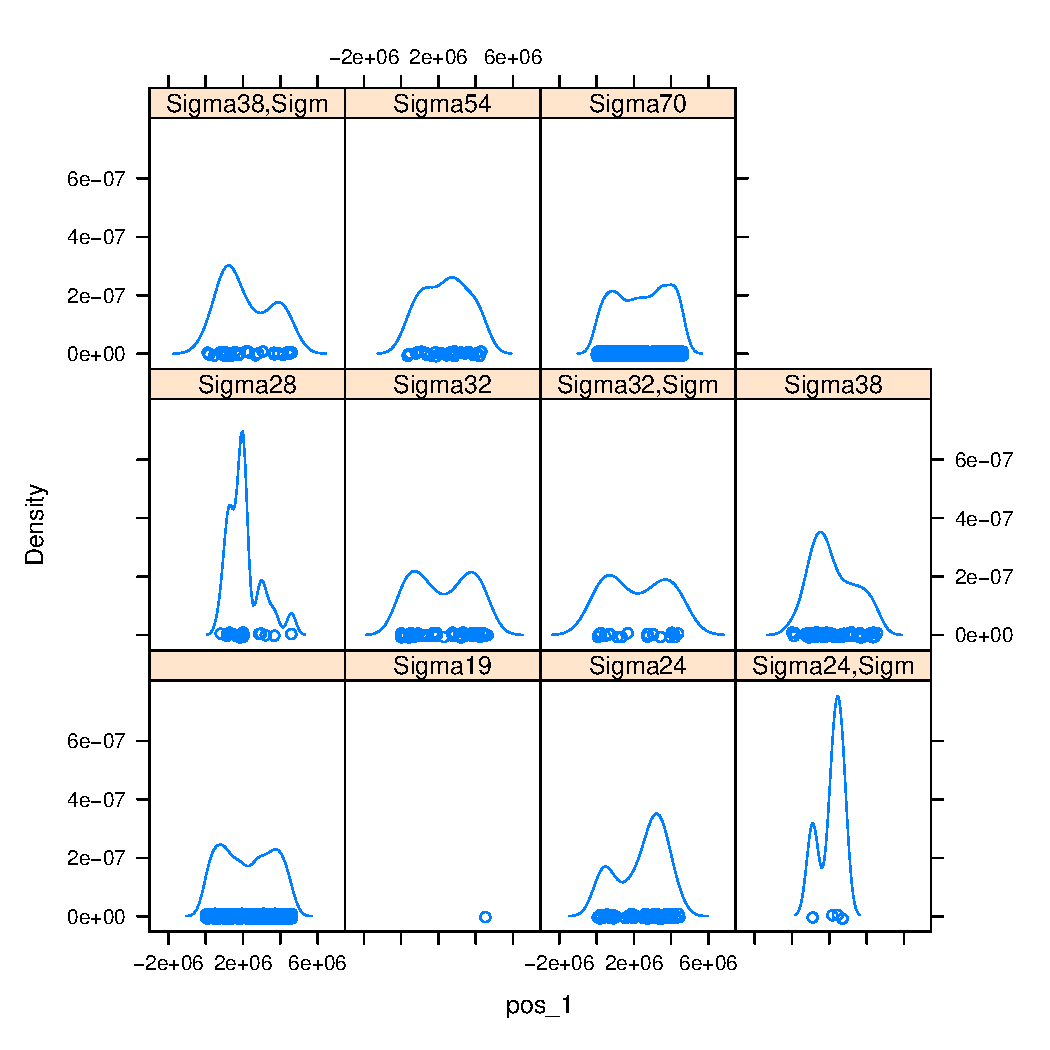
\includegraphics[width=1\textwidth]{imagen.pdf}  
  \caption{Densityplot for the pos\_1 by promoter\_sigma type}
  \end{figure}
  
  \item If you don't have your own database, let me know.
  \end{enumerate}


\end{document}
